\documentclass[a4paper]{oblivoir}
\usepackage{amsmath,amssymb,kotex,kswrapfig,mdframed,paralist}
\usepackage{fapapersize}
\usefapapersize{210mm,297mm,20mm,*,20mm,*}

\usepackage{tabto,pifont}
\TabPositions{0.2\textwidth,0.4\textwidth,0.6\textwidth,0.8\textwidth}
\newcommand\tabb[5]{\par\noindent
\ding{172}\:{\ensuremath{#1}}
\tab\ding{173}\:\:{\ensuremath{#2}}
\tab\ding{174}\:\:{\ensuremath{#3}}
\tab\ding{175}\:\:{\ensuremath{#4}}
\tab\ding{176}\:\:{\ensuremath{#5}}}

\usepackage{graphicx}

%\pagestyle{empty}

%%% Counters
\newcounter{num}

%%% Commands
\newcommand\prob[1]
{\vs\bigskip\bigskip\par\noindent\stepcounter{num} \textbf{문제 \thenum) #1}\par\noindent}

\newcommand\pb[1]{\ensuremath{\fbox{\phantom{#1}}}}

\newcommand\ba{\ensuremath{\:|\:}}

\newcommand\vs[1]{\vspace{40pt}}

\newcommand\an[1]{\bigskip\par\noindent\textbf{문제 #1)}\par\noindent}

%%% Meta Commands
\let\oldsection\section
\renewcommand\section{\clearpage\oldsection}

\let\emph\textsf

\begin{document}
\begin{center}
\LARGE준영, 미니테스트 22
\end{center}
\begin{flushright}
날짜 : 2017년 \(\pb3\)월 \(\pb{10}\)일 \(\pb{월}\)요일
,\qquad
제한시간 : \pb{17년}분
,\qquad
점수 : \pb{20} / \pb{20}
\end{flushright}

%
\prob{}
함수 \(f(x)\)의 한 부정적분을 \(F(x)\)라고 할 때, <보기>에서 옳은 것만을 있는 대로 고른 것은?
(단, \(C\)는 적분상수)
\begin{mdframed}[frametitle=<보기>]
ㄱ. \(\displaystyle\int\{1+f(x)\}\,dx=x+F(x)+C\)\\
ㄴ. \(\displaystyle\int F(x)f(x)\,dx=\frac12\{F(x)\}^2+C\)\\
ㄷ. \(\displaystyle\int\{xf(x)+F(x)\}\,dx=xF(x)+C\)\\
\end{mdframed}
\par\bigskip
\tabb{\text{ㄱ}}{\textㄷ}{\text{ㄱ, ㄴ}}{\text{ㄴ, ㄷ}}{\text{ㄱ, ㄴ, ㄷ}}

%
\prob{}
\(\displaystyle
\log_2\left(\frac d{dx}\int4\,dx\right)+2\log_2\left(\frac d{dx}\int8\,dx\right)
\)
의 값을 구하여라.
\par\bigskip
\tabb2468{10}

%
\prob{}
삼차함수 \(f(x)\)의 도함수가 \(f'(x)=x(x+1)\)일 때, \(f(x)\)의 극댓값과 극솟값의 차는?
\tabb{\frac16}{\frac13}{\frac12}{\frac23}{\frac56}

%
\prob{}
다음 중 항상 옳은 것은?
\par\smallskip\ding{172}
\(\displaystyle\int0\,dx=0\)
\par\smallskip\ding{173}
\(\displaystyle\int x\,dx=\int y\,dy\)\\
\par\smallskip\ding{174}
\(\displaystyle\int\{f(x)g(x)\}\,dx=\left(\int f(x)\,dx\right)\left(\int g(x)\,dx\right)\)\\
\par\smallskip\ding{175}
\(\displaystyle\int f(x)\,dx=\displaystyle\int g(x)\,dx\)이면 \(f(x)=g(x)\)\\
\par\smallskip\ding{176}
\(f'(x)=g'(x)\)이면 \(\displaystyle\int f'(x)\,dx=\int g'(x)\,dx\)

%
\prob{}
곡선 \(y=f(x)\) 위의 점 \((x,f(x))\)에서의 접선의 기울기가 \(3x^2+2x+2\)이고 이 곡선이 점 \((0,-4)\)를 지난다.
곡선 \(y=f(x)\)가 \(x\)축과 만나는 점의 좌표가 \((k,0)\)일 때, 상수 \(k\)의 값을 구하시오.
\par\bigskip
\tabb01234

%
\prob{}
미분가능한 함수 \(f(x)\)가 모든 실수 \(x\), \(y\)에 대하여
\[f(x+y)=f(x)+f(y)+2xy-2\]
을 만족시킨다.
\(\displaystyle\lim_{x\to1}\frac{f(x)-f'(x)-1}{x^2-1}=8\)
일 때, \(f(2)\)의 값을 구하시오.
\par\bigskip
\tabb{34}{38}{42}{46}{50}

%
\prob{}
다항함수 \(f(x)\)가 모든 실수 \(x\)에 대하여
\[x^4-4x^3+x^2+xf(x)=\int_1^xf(t)\,dt\]
를 만족시킬 때, \(f(-1)\)의 값은?
\tabb{\frac{22}3}{\frac{23}3}8{\frac{25}3}{\frac{26}3}

%
\prob{}
함수 \(f(x)=-x^3+3x^2+5\)에 대하여\\
\(f'(\alpha)=f'(\beta)=0\)일 때, \(\displaystyle\int_\alpha^\beta f'(x)\,dx\)의 값을 구하시오.
(단, \(\alpha\), \(\beta\)는 \(\alpha<\beta\)인 상수이다.)
\par\bigskip
\tabb12345

%
\prob{}
연속함수 \(f(x)\)가
\[\int_0^{-2}f(x)\,dx=-4,\quad\int_0^3f(x)\,dx=5,\quad\int_3^4f(x)\,dx=7\]
을 만족시킬 때, \(\displaystyle\int_{-2}^4f(x)\,dx\)의 값은?
\par\bigskip
\tabb8{10}{12}{14}{16}

%
\prob{}
\begin{minipage}{0.5\textwidth}
\(0\le x\le3\)에서 정의된 함수 \(y=f(x)\)의 그래프가 그림과 같을 때, \(\displaystyle\int_0^3xf(x)\,dx=a\)이다.
\(30a\)의 값을 구하시오.
\end{minipage}
\begin{minipage}{0.4\textwidth}
\centering
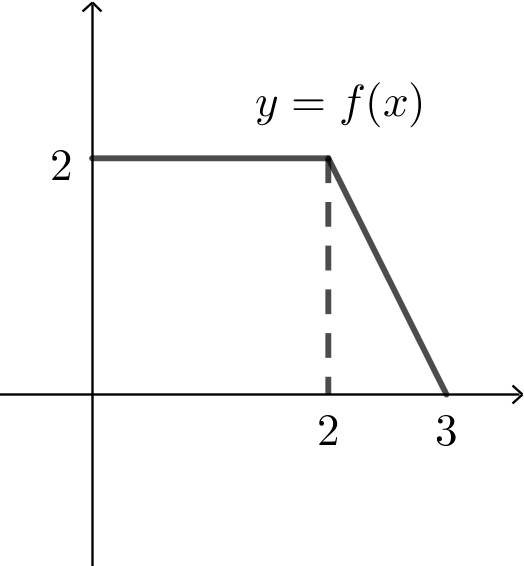
\includegraphics[width=0.5\textwidth]{10}
\end{minipage}
\tabb{150}{160}{170}{180}{190}

%
\prob{}
모든 실수 \(x\)에 대하여 함수 \(f(x)\)가 \(f(x)=f(x+4)\)를 만족시킬 때, 다음 중 정적분 \(\displaystyle\int_1^3f(x-1)\,dx\)와 항상 같은 값을 갖는 것은?
\par\bigskip
\tabb
{\displaystyle\int_{10}^{12}f(x)\,dx}
{\displaystyle\int_{12}^{10}f(x)\,dx}
{\displaystyle\int_{11}^{13}f(x)\,dx}
{\displaystyle\int_{13}^{11}f(x)\,dx}
{\displaystyle\int_{12}^{14}f(x)\,dx}

%
\prob{}
다항함수 \(f(x)\)가 모든 실수 \(x\)에 대하여
\[f(x)=3x^2+x\int_0^1f(t)\,dt\]
을 만족시킬 때, \(\displaystyle\lim_{x\to1}\frac{f(x^2)-f(1)}{x-1}\)의 값을 구하시오.
\par\bigskip
\tabb48{16}{20}{24}

%
\prob{}
\(\displaystyle\lim_{n\to\infty}\frac4n\left[
\left(1+\frac2n\right)^3+\left(1+\frac4n\right)^3+\left(1+\frac6n\right)^3
+\cdots+\left(1+\frac{2n}n\right)^3\right]
\)의 값을 구하시오.
\par\bigskip
\tabb{10}{20}{30}{40}{50}

%
\prob{}
\(\displaystyle\lim_{n\to\infty}\displaystyle\frac{(n+1)^4+(n+2)^4+\cdots+(2n)^4}{1^4+2^4+\cdots+n^4}\)의 값은?
\par\bigskip
\tabb{31}{33}{35}{37}{39}

\end{document}